
%%%%%%%%%%%%%%%%%%%%%%%%%%%%%%%%%%%%%%%%%%%%%%%%%%%%%%%%%%%%%%%%%%%%%%%%%%%%%%%%
%2345678901234567890123456789012345678901234567890123456789012345678901234567890
%        1         2         3         4         5         6         7         8
% THESIS CHAPTER

%\section*{Visualisations}

% short summary of the chapter

\chapter{Visualisation Interface}
This chapter details the visualisations that have been implemented, the various components involved and some of the approaches that were briefly taken but were ultimately changed or not implemented.


\begin{figure}[h!]
  \begin{center}
  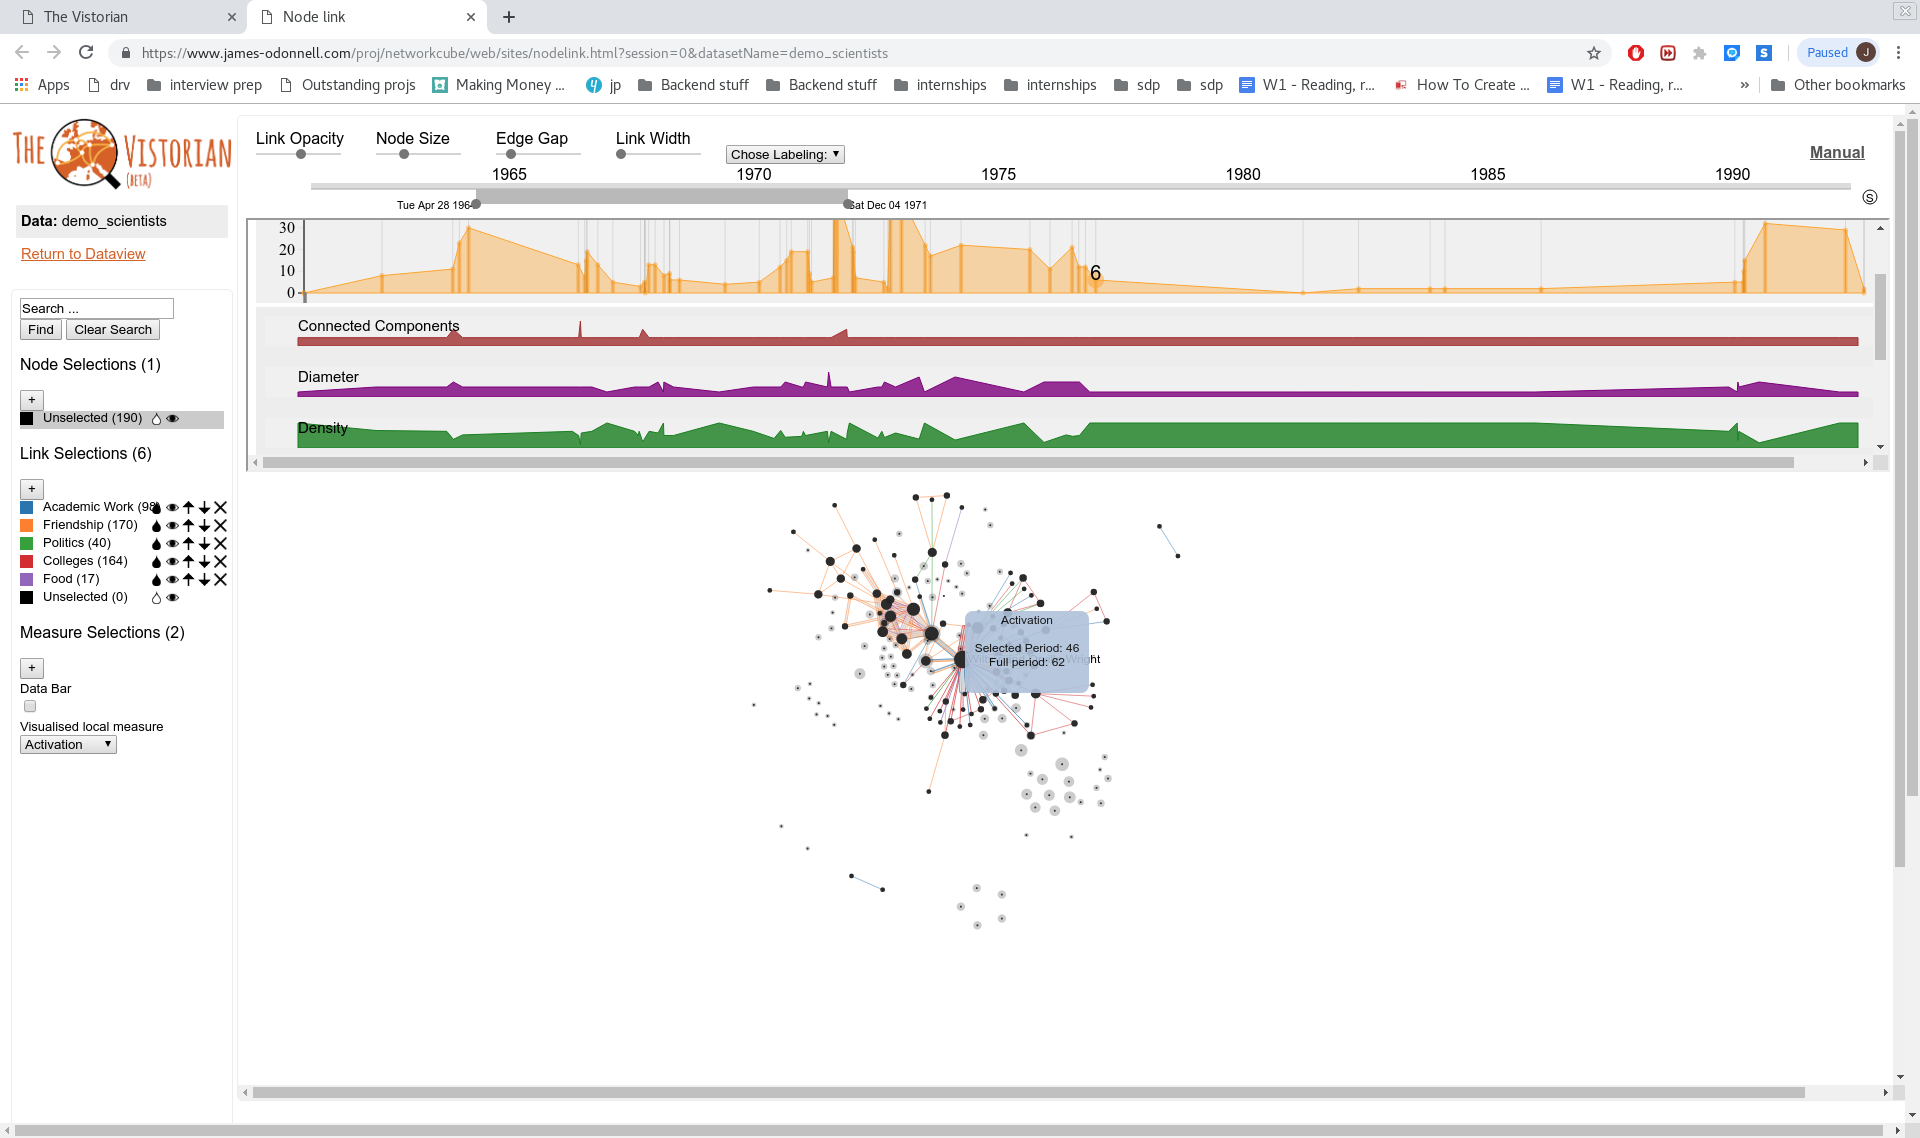
\includegraphics[trim={0, 0, 0, 3.5cm}, clip, width=140mm]{./Figures/vistorianNewFull.png}
  \caption{Final user interface}
  \label{fig:vistorianNewFull}
  \end{center}
\end{figure}

\subsection{The Databar}

\begin{center}
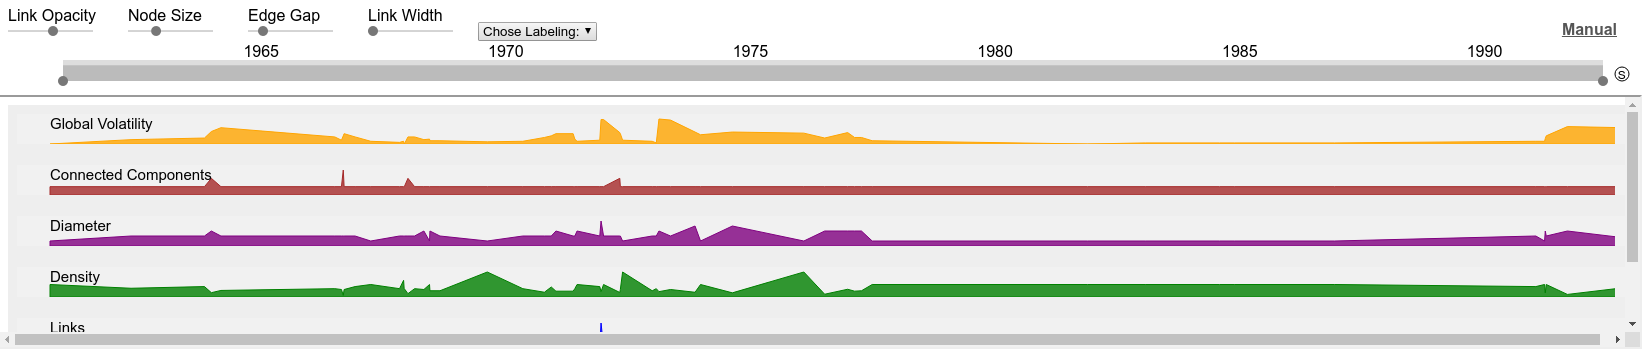
\includegraphics[trim={0 0 0 0}, width=140mm]{./Figures/databar.png}
\end{center}

The Databar holds the visualisation graphs for global measures. I decided to place it along the top of the window because it would line up nicely with the pre-existing timeline which could then double as the x-axis label - saving valuable screen space.
The databar is highly interactive. Each graph is initially collapsed and can then be expanded by clicking. As more measures were added I realised that it wouldn't be possible to both provide enough detail in every graph and also facilitate easy comparison without taking up most of the screen real estate. Collapsing and expanding the graphs solved this problem. The databar was designed to be readily extensible and only needs to be provided with a list of values the same length as the number of time frames. It then maps each value to the corresponding time frame to produce the co-ordinate values for the ridgeline. 

\begin{center}
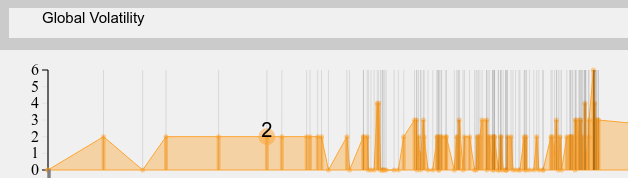
\includegraphics[trim={0 0 0 0}, width=140mm]{./Figures/margueriteGlobalVolatility.png}
\end{center}
A d3 scale is used to provide the y axis labels seen on the left of the expanded graph. Moving the mouse across the screen causes a cursor to track along the ridgeline of the graph. The y-label at that point is shown on the tracker. This was originally done when the graphs weren't expandable to remove the need for an axis and save space, however it was found to be useful for tightly clumped values and for data with some small step sizes.

\begin{center}
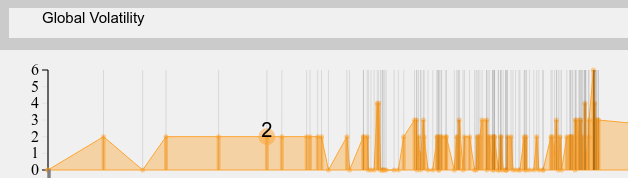
\includegraphics[trim={5cm, 0, 9cm, 2cm},clip, width=70mm]{./Figures/margueriteGlobalVolatility.png}
\end{center}
The vertical lines indicate a timestep/change in the graph. This was orignally simply intended to make it easier for the user to  compare graphs vertically, however an additional and powerful benefit is that it allows the user to  easily finding time periods of high or low activity. The vertical lines are thicker and of the same colour as the graph when inside it's area to emphasise the fact that these are the only points there is information for, and that the connecting ridge-line is interpolated between them.
Finally, graphs can be reordered for easy comparison using click and drag as there is not enough screen space to see all graphs at once, even compressed.

\subsection{Bookmarks Bar Additions}
\begin{figure}
  \begin{center}
  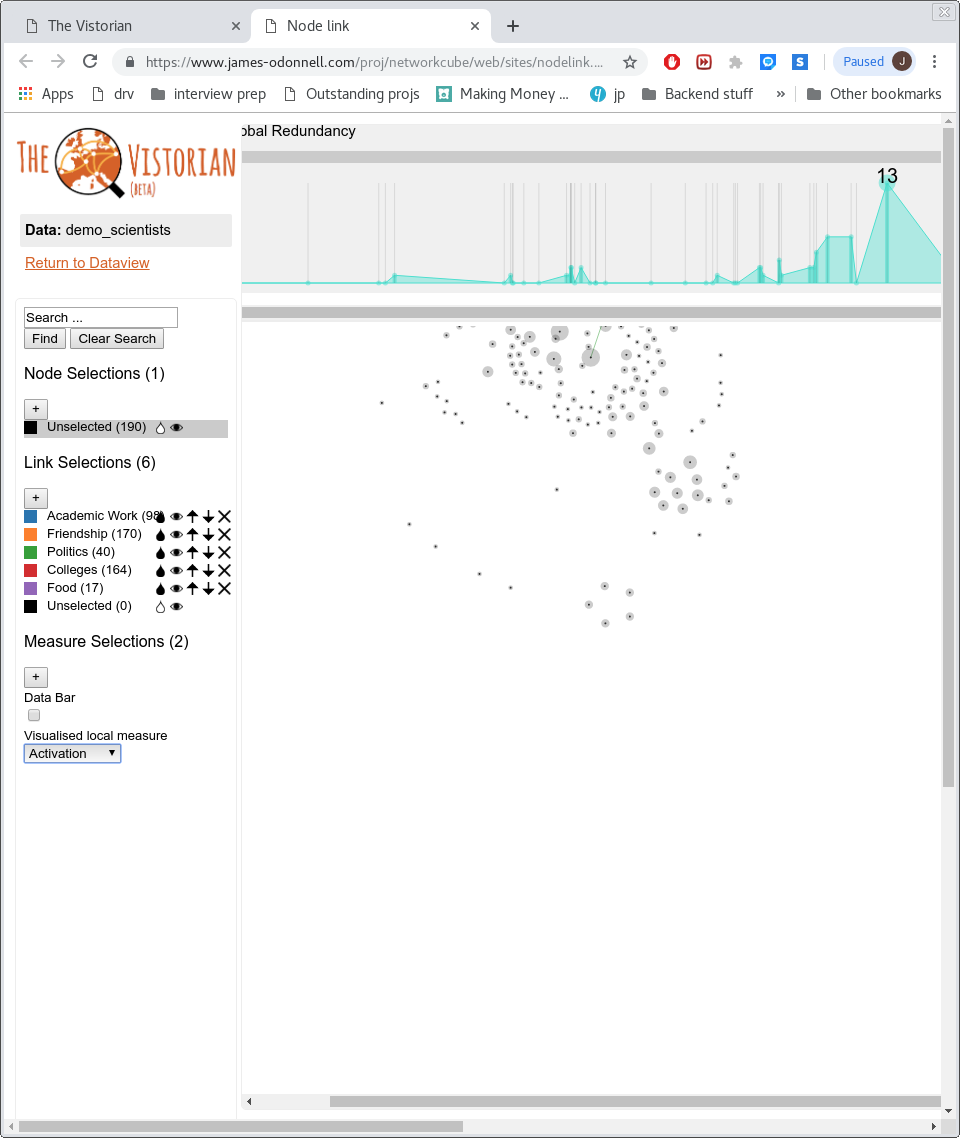
\includegraphics[trim={0, 12cm, 20cm, 22cm},clip, width=140mm]{./Figures/bookmarksbar.png}
  \caption{Bookmarks Bar Measures Extension}
  \label{fig:bookmarksbar}
  \end{center}
\end{figure}

The bookmarks bar has been extended with a checkbox to show or hide the databar and a dropdown to pick between local measures, shown in Figure \ref{fig:bookmarksbar}. It defaults to centrality.

%%%%%%%%%%%%%%%%%%%%%%%%%%%%%%%%%%%%%%%%%%%%%%%%%%%%%%%%%%%%%%%%%%%%%%%%%%%%%%%%%%%%%%%%%%%%%%%%%%%%%%%%%%%%%%%
%LOCAL MEASURE VISUALISATION.
%%%%%%%%%%%%%%%%%%%%%%%%%%%%%%%%%%%%%%%%%%%%%%%%%%%%%%%%%%%%%%%%%%%%%%%%%%%%%%%%%%%%%%%%%%%%%%%%%%%%%%%%%%%%%%%
\section{Local Measure Hoverover}
\label{sec:localMeasureVis}
To save screen space and reduce visual complexity, the precise values of a node's local measures given the selected time period are only shown on hover over. For the purposes of this report, the local measures are degree centrality and local volatility. However the implementation is easily extensible, allowing for more local measures to be quickly visualised.

Initially, local volatility was visualised using 'spikes', where more spikes indicated higher local volatility. Other methods were considered, vibration matches with the mental image of volatility but would be too distracting to the eye. Dotted rings with larger diameter indicating higher local volatility were considered but had too much potential for confusing overlap. Colours were originally used but could be misconstrued as relating to the edge colours. 
However as more local measures were added the spikes made less sense. They were also somewhat difficult to count on smaller nodes.

\begin{center}
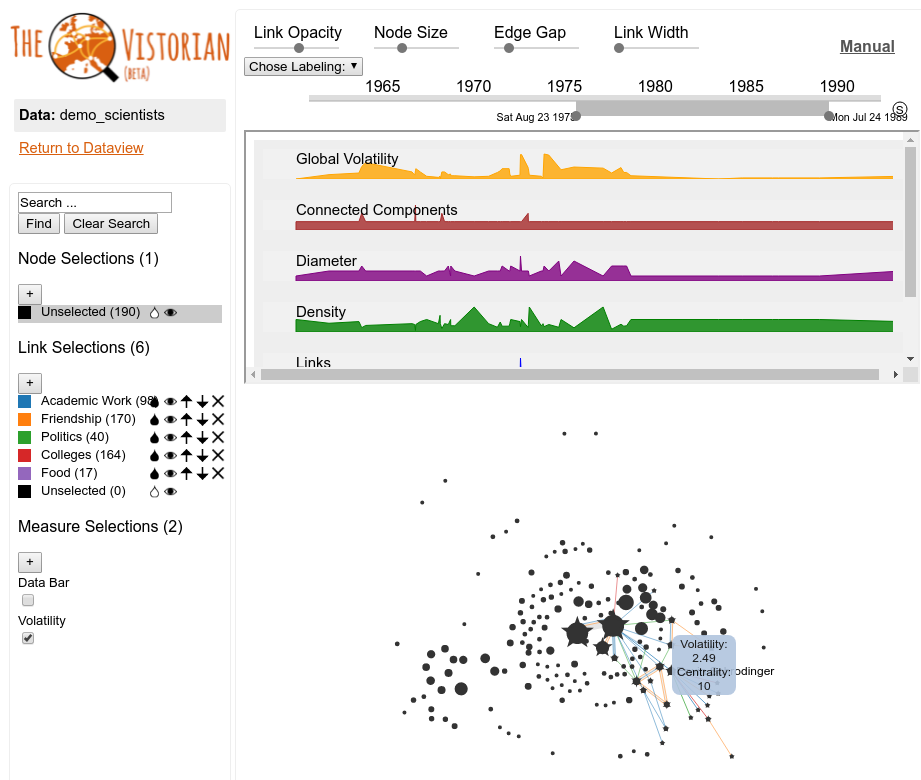
\includegraphics[trim={9cm, 0, 0, 14cm}, clip, width=140mm]{./Figures/finalUI.png}
\end{center}

Local activation, redundancy, volatility and centrality are all visualised in the same way - as the radius of the node in the network visualisation. The drop down in the bookmarks bar is used to select between them. The values are calculated for each node and the nodes radius is then calculated as the log of double the measures value, plus one. The values are doubled to give more visual separation which is hampered by the log scale. The "+1" is added so that nodes always have a radius to avoid breaking the user's mental map \cite{BLANK}.

To aid the user further, a lighter grey circle or 'halo' of a fixed radius is shown behind each node'. It's radius is calculated given the active local measure as that measures value over the full time frame. This allows users to see how a smaller window of time differs from the full time period. It was considered to use the maximum value that the selected measure ever takes for each given node, however this would require considerable initial computation as all pairs of start and end times would have to be considered for every single node. This solution doesn't work for redundancy as there are no redundant nodes over the full period.

\begin{figure}[h!]
  \begin{center}
  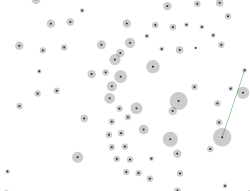
\includegraphics[trim={0, 0, 0, 0}, width=70mm]{./Figures/greyCircles.png}
  \caption{Fixed nodes 'halos'}
  \label{fig:greyCircles}
  \end{center}
\end{figure}









